\section{Part C.}
\begin{figure*}[t]
\begin{subfigure}[t]{0.30\linewidth}
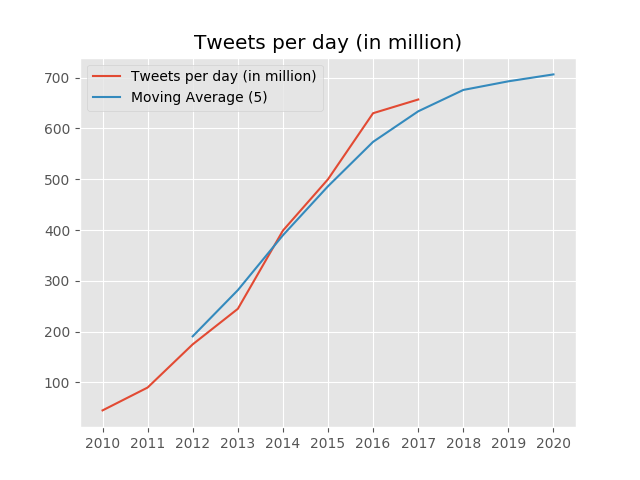
\includegraphics[width=\linewidth ]{fig/tweets_ma.png}
\caption{{\footnotesize Moving Average with window 5.}}\vspace{-2mm}
\label{fig:pla1}
\end{subfigure}
\begin{subfigure}[t]{0.30\linewidth}
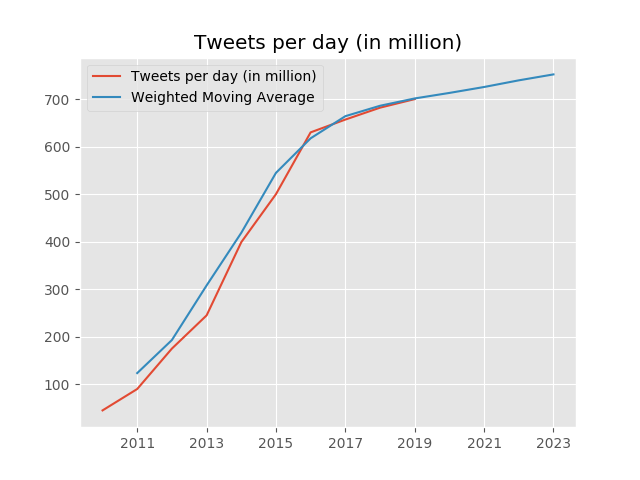
\includegraphics[width=\linewidth ]{fig/tweets_wma.png}
\caption{{\footnotesize Weighted Moving Average with window 3 (0.5, 0.3, 0.2).}}\vspace{-2mm}
\label{fig:pla2}
\end{subfigure}
\begin{subfigure}[t]{0.30\linewidth}
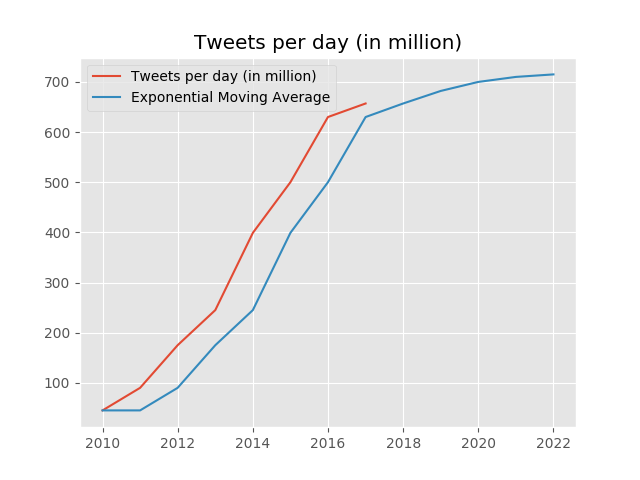
\includegraphics[width=\linewidth ]{fig/tweets_ema.png}
\caption{{\footnotesize Exponential Moving Average with $\alpha = 0.9$.}}\vspace{-2mm}
\label{fig:pla2}
\end{subfigure}
\caption{Predicting tweets per day from 2019-2022.}\vspace{-2mm}
\label{fig:tweet_day}
\end{figure*}

\begin{figure*}[t]
\begin{subfigure}[t]{0.30\linewidth}
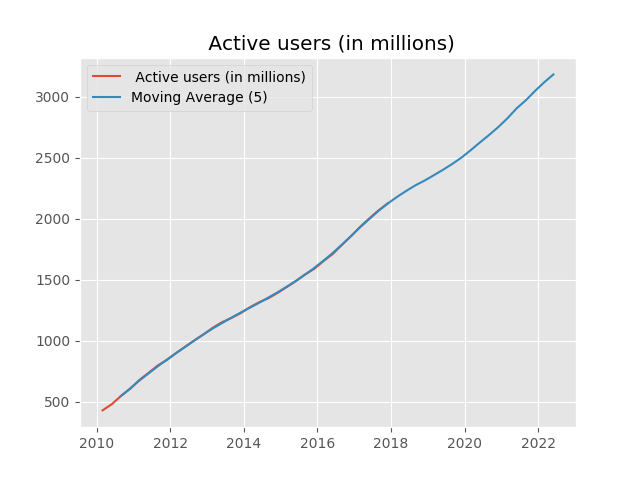
\includegraphics[width=\linewidth ]{fig/fb_ma.png}
\caption{{\footnotesize Moving Average with window 5.}}\vspace{-2mm}
\label{fig:pla1}
\end{subfigure}
\begin{subfigure}[t]{0.30\linewidth}
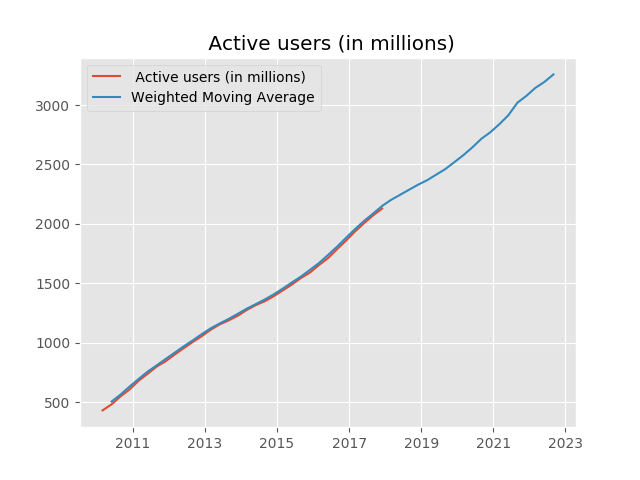
\includegraphics[width=\linewidth ]{fig/fb_wma.png}
\caption{{\footnotesize Weighted Moving Average with window 3 (0.5, 0.3, 0.2).}}\vspace{-2mm}
\label{fig:pla2}
\end{subfigure}
\begin{subfigure}[t]{0.30\linewidth}
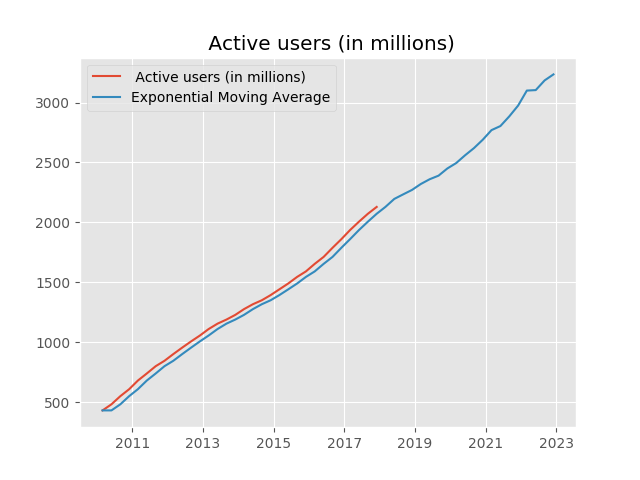
\includegraphics[width=\linewidth ]{fig/fb_ema.png}
\caption{{\footnotesize Exponential Moving Average with $\alpha = 0.9$.}}\vspace{-2mm}
\label{fig:pla2}
\end{subfigure}
\caption{Predicting Facebook monthly average users from 2019-2022.}\vspace{-2mm}
\label{fig:fb_users}
\end{figure*}

\begin{figure*}[t]
\begin{subfigure}[t]{0.30\linewidth}
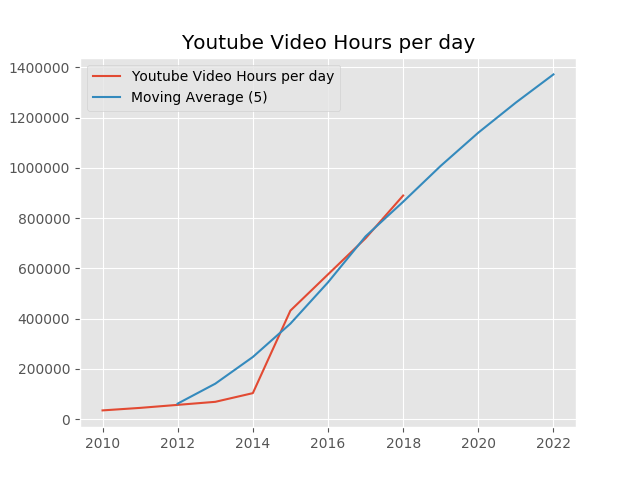
\includegraphics[width=\linewidth ]{fig/yt_ma.png}
\caption{{\footnotesize Moving Average with window 5.}}\vspace{-2mm}
\label{fig:pla1}
\end{subfigure}
\begin{subfigure}[t]{0.30\linewidth}
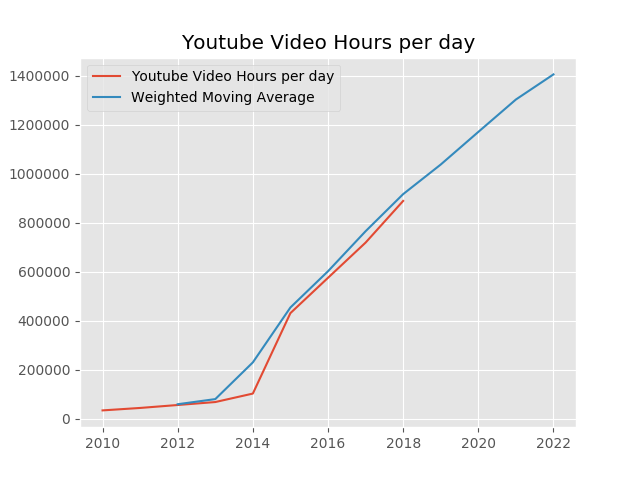
\includegraphics[width=\linewidth ]{fig/yt_wma.png}
\caption{{\footnotesize Weighted Moving Average with window 4 (0.5, 0.35, 0.05,0.05).}}\vspace{-2mm}
\label{fig:pla2}
\end{subfigure}
\begin{subfigure}[t]{0.30\linewidth}
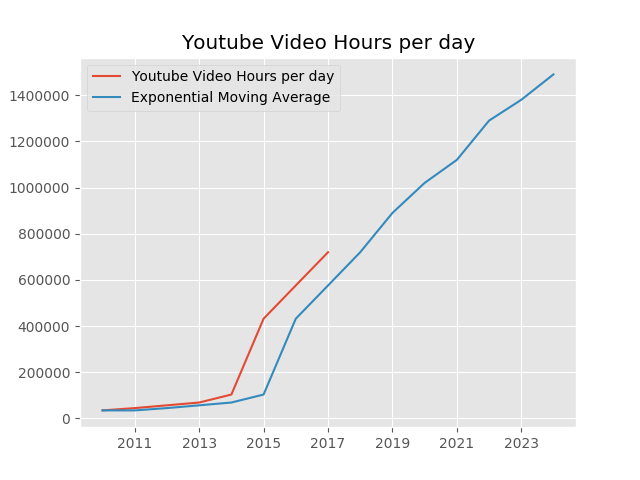
\includegraphics[width=\linewidth ]{fig/yt_ema.png}
\caption{{\footnotesize Exponential Moving Average with $\alpha = 1.0$.}}\vspace{-2mm}
\label{fig:pla2}
\end{subfigure}
\caption{Predicting Youtube video upload hours from 2019-2022.}\vspace{-2mm}
\label{fig:youtube_upload}
\end{figure*}



\subsection*{Predicting future:}
As mentioned in Section \ref{part_a} that there is no true evident relation between the amount of social media data available with companies and data available for public research; except for Twitter. Hence, we will try to predict how much social media data will be available in 2022 within the Twitter.
Also the fact that I have limited amount of information from Table \ref{table:users} and Table \ref{table:media_units}, it will be wise to start with a simple forecasting methods. Also it is very common for extremely simple methods like forecast with historical average to outperform more complex methods \cite{simple_forecast}. This statement is even more likely true for short time series.



To start with the basic forecasting model we might consider historical {\em mean model} which assumes that the time series consists of independently and identically distributed (``i.i.d.") values, as if each observation is randomly drawn from the same population. Under this assumption, the next value should be predicted to be equal to the historical sample mean if the goal is to minimize mean squared error. I tried a bunch of experiment with {\em mean model} and it appeared to be working well with relatively moderate mean squared error.

I avoided linear trend model as it is not a very {\em robust} model for time-series forcasting \cite{nau2014review}. Since I have the
priori knowledge of the series that has a positive trend or zero trend I can use a moving
average model that puts more weight on the most recent values than to use a linear trend model
with a {\em not very significant} trend estimate. With this notion I tried the {\em moving average model} to forecast the tweets per day metric for 2022. I tried more forecasting methods with {\em weighted moving average} and {\em exponential moving average model }. Figure \ref{fig:tweet_day} presents all the forecasts for tweets per day metric till 2022 \footnote{\href{https://github.com/debjyoti385/MovingAverageForecasting}{github.com/debjyoti385/MovingAverageForecasting}}.

Complex models like {\em ARMA (AutoRegressive Moving Average)} and {\em ARIMA (AutoRegressive  Integrated Moving Average)} models  did not do well (validating with small train test data).

From the prediction in Figure \ref{fig:tweet_day}, we find that twitter will generate around 730 million tweets every day in average. That is almost 2.4 terabytes of tweet data withput media.

Similar forecasting applied on Facebook monthly active users in Figure \ref{fig:fb_users} reveals that almost 3000 million people will be active in Facebook by the end of 2022. From Youtube's hourly video upload data, it is predicted that in 2022 users will upload 1.4 million hours of video everyday \ref{fig:youtube_upload}.




%%% Local Variables:
%%% mode: latex
%%% TeX-master: "main"
%%% End:
